\tikzset{every picture/.style={line width=0.75pt}} %set default line width to 0.75pt        

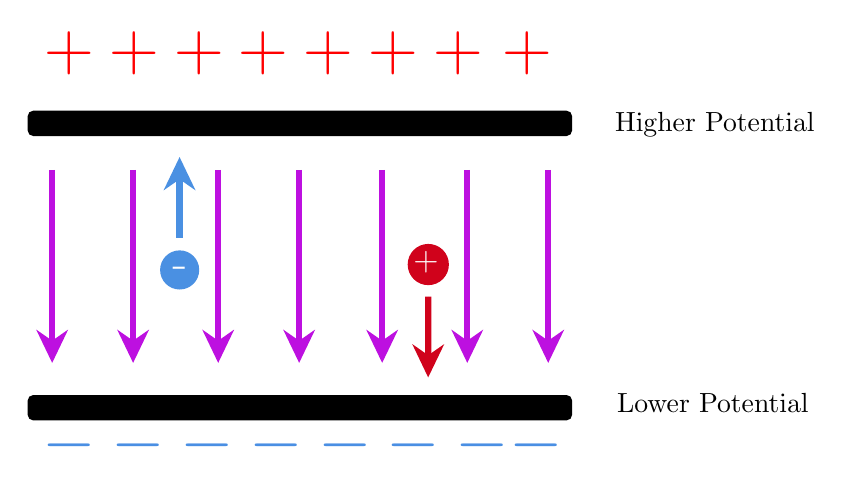
\begin{tikzpicture}[x=0.75pt,y=0.75pt,yscale=-1,xscale=1]
%uncomment if require: \path (0,300); %set diagram left start at 0, and has height of 300

%Rounded Rect [id:dp26809755411510916] 
    \draw  [fill={rgb, 255:red, 0; green, 0; blue, 0 }  ,fill opacity=1 ] (100,75.24) .. controls (100,74) and (101,73) .. (102.24,73) -- (359.06,73) .. controls (360.3,73) and (361.3,74) .. (361.3,75.24) -- (361.3,81.96) .. controls (361.3,83.2) and (360.3,84.2) .. (359.06,84.2) -- (102.24,84.2) .. controls (101,84.2) and (100,83.2) .. (100,81.96) -- cycle ;
%Rounded Rect [id:dp7927549373308511] 
    \draw  [fill={rgb, 255:red, 0; green, 0; blue, 0 }  ,fill opacity=1 ] (100,212.24) .. controls (100,211) and (101,210) .. (102.24,210) -- (359.06,210) .. controls (360.3,210) and (361.3,211) .. (361.3,212.24) -- (361.3,218.96) .. controls (361.3,220.2) and (360.3,221.2) .. (359.06,221.2) -- (102.24,221.2) .. controls (101,221.2) and (100,220.2) .. (100,218.96) -- cycle ;
%Straight Lines [id:da2975639375446937] 
    \draw [color={rgb, 255:red, 189; green, 16; blue, 224 }  ,draw opacity=1 ][line width=2.25]    (111.3,101) -- (111.3,189) ;
    \draw [shift={(111.3,194)}, rotate = 270] [fill={rgb, 255:red, 189; green, 16; blue, 224 }  ,fill opacity=1 ][line width=0.08]  [draw opacity=0] (16.07,-7.72) -- (0,0) -- (16.07,7.72) -- (10.67,0) -- cycle ;
%Straight Lines [id:da1334330283651397] 
    \draw [color={rgb, 255:red, 189; green, 16; blue, 224 }  ,draw opacity=1 ][line width=2.25]    (150.3,101) -- (150.3,189) ;
    \draw [shift={(150.3,194)}, rotate = 270] [fill={rgb, 255:red, 189; green, 16; blue, 224 }  ,fill opacity=1 ][line width=0.08]  [draw opacity=0] (16.07,-7.72) -- (0,0) -- (16.07,7.72) -- (10.67,0) -- cycle ;
%Straight Lines [id:da11942725415140942] 
    \draw [color={rgb, 255:red, 189; green, 16; blue, 224 }  ,draw opacity=1 ][line width=2.25]    (191.3,101) -- (191.3,189) ;
    \draw [shift={(191.3,194)}, rotate = 270] [fill={rgb, 255:red, 189; green, 16; blue, 224 }  ,fill opacity=1 ][line width=0.08]  [draw opacity=0] (16.07,-7.72) -- (0,0) -- (16.07,7.72) -- (10.67,0) -- cycle ;
%Straight Lines [id:da6347096895979325] 
    \draw [color={rgb, 255:red, 189; green, 16; blue, 224 }  ,draw opacity=1 ][line width=2.25]    (230.3,101) -- (230.3,189) ;
    \draw [shift={(230.3,194)}, rotate = 270] [fill={rgb, 255:red, 189; green, 16; blue, 224 }  ,fill opacity=1 ][line width=0.08]  [draw opacity=0] (16.07,-7.72) -- (0,0) -- (16.07,7.72) -- (10.67,0) -- cycle ;
%Straight Lines [id:da628279138260976] 
    \draw [color={rgb, 255:red, 189; green, 16; blue, 224 }  ,draw opacity=1 ][line width=2.25]    (270.3,101) -- (270.3,189) ;
    \draw [shift={(270.3,194)}, rotate = 270] [fill={rgb, 255:red, 189; green, 16; blue, 224 }  ,fill opacity=1 ][line width=0.08]  [draw opacity=0] (16.07,-7.72) -- (0,0) -- (16.07,7.72) -- (10.67,0) -- cycle ;
%Straight Lines [id:da8819882926387512] 
    \draw [color={rgb, 255:red, 189; green, 16; blue, 224 }  ,draw opacity=1 ][line width=2.25]    (311.3,101) -- (311.3,189) ;
    \draw [shift={(311.3,194)}, rotate = 270] [fill={rgb, 255:red, 189; green, 16; blue, 224 }  ,fill opacity=1 ][line width=0.08]  [draw opacity=0] (16.07,-7.72) -- (0,0) -- (16.07,7.72) -- (10.67,0) -- cycle ;
%Straight Lines [id:da5899822516769986] 
    \draw [color={rgb, 255:red, 189; green, 16; blue, 224 }  ,draw opacity=1 ][line width=2.25]    (350.3,101) -- (350.3,189) ;
    \draw [shift={(350.3,194)}, rotate = 270] [fill={rgb, 255:red, 189; green, 16; blue, 224 }  ,fill opacity=1 ][line width=0.08]  [draw opacity=0] (16.07,-7.72) -- (0,0) -- (16.07,7.72) -- (10.67,0) -- cycle ;
%Shape: Ellipse [id:dp7796258826987774] 
    \draw  [draw opacity=0][fill={rgb, 255:red, 74; green, 144; blue, 226 }  ,fill opacity=1 ] (163.3,149.27) .. controls (163.27,144.06) and (167.47,139.82) .. (172.68,139.79) .. controls (177.88,139.77) and (182.12,143.97) .. (182.15,149.17) .. controls (182.18,154.38) and (177.98,158.62) .. (172.77,158.65) .. controls (167.57,158.67) and (163.33,154.47) .. (163.3,149.27) -- cycle ;
%Straight Lines [id:da4888240085287785] 
    \draw [color={rgb, 255:red, 74; green, 144; blue, 226 }  ,draw opacity=1 ][line width=2.25]    (172.68,133.75) -- (172.68,99.84) ;
    \draw [shift={(172.68,94.84)}, rotate = 450] [fill={rgb, 255:red, 74; green, 144; blue, 226 }  ,fill opacity=1 ][line width=0.08]  [draw opacity=0] (16.07,-7.72) -- (0,0) -- (16.07,7.72) -- (10.67,0) -- cycle ;
%Shape: Ellipse [id:dp3890055755107731] 
    \draw  [color={rgb, 255:red, 208; green, 2; blue, 27 }  ,draw opacity=1 ][fill={rgb, 255:red, 208; green, 2; blue, 27 }  ,fill opacity=1 ] (301.94,146.58) .. controls (301.95,151.79) and (297.75,156.02) .. (292.54,156.04) .. controls (287.34,156.06) and (283.1,151.85) .. (283.09,146.65) .. controls (283.07,141.44) and (287.27,137.21) .. (292.48,137.19) .. controls (297.69,137.17) and (301.92,141.38) .. (301.94,146.58) -- cycle ;
%Straight Lines [id:da9866534236439359] 
    \draw [color={rgb, 255:red, 208; green, 2; blue, 27 }  ,draw opacity=1 ][fill={rgb, 255:red, 208; green, 2; blue, 27 }  ,fill opacity=1 ][line width=2.25]    (292.53,162.09) -- (292.47,196) ;
    \draw [shift={(292.46,201)}, rotate = 270.1] [fill={rgb, 255:red, 208; green, 2; blue, 27 }  ,fill opacity=1 ][line width=0.08]  [draw opacity=0] (16.07,-7.72) -- (0,0) -- (16.07,7.72) -- (10.67,0) -- cycle ;

% Text Node
    \draw (106,33) node [anchor=north west][inner sep=0.75pt]   [align=left] {{\Huge \textcolor[rgb]{1,0,0}{$+ + + + + + +\; + $}}};
% Text Node
    \draw (105.24,221) node [anchor=north west][inner sep=0.75pt]   [align=left] {{\Huge \textcolor[rgb]{0.29,0.56,0.89}{$-------- $}}};
% Text Node
    \draw (166.81+1,142) node [anchor=north west][inner sep=0.75pt]   [align=left] {\textcolor[rgb]{1,1,1}{{\LARGE -}}};
% Text Node
    \draw (283+.8,137+2) node [anchor=north west][inner sep=0.75pt]   [align=left] {\textcolor[rgb]{1,1,1}{{\large +}}};
% Text Node
    \draw (381,72) node [anchor=north west][inner sep=0.75pt]   [align=left] {Higher Potential};
% Text Node
    \draw (382,207) node [anchor=north west][inner sep=0.75pt]   [align=left] {Lower Potential};


\end{tikzpicture}